%% Included in decks: slidemage-manual
%%

% SlideMage manual, chapter "Working in SlideMage": the slide-level buttons of
% the slide editor (top row) and its two AI buttons. The strip is a crop of the
% editor's two button rows (tools/manual/make_screenshots.py).
\setSlideVersion{1-0-0}
\begin{standardframe}{Managing a slide in the editor}
	\small
	These buttons act on the whole slide, not its text; several also update the decks that use it.
	\par\smallskip
	\centering
	{\setlength{\fboxsep}{0pt}\fcolorbox{c_primary_gray}{white}{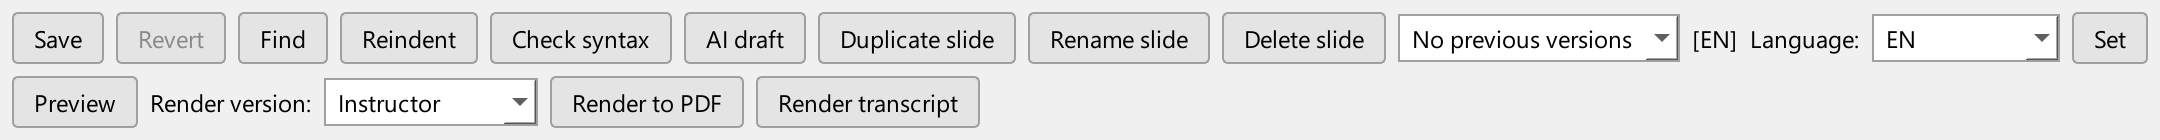
\includegraphics[width=\dimexpr0.98\linewidth-0.8pt\relax]{media/screenshot-slidemage-slide-editor-buttons.png}}}
	\par\smallskip
	\raggedright
	\begin{columns}[T,onlytextwidth]
		\begin{column}{0.6\linewidth}
			\textbf{The slide}
			\shrinklists{2}
			\begin{itemize}
				\item \emph{Save}: writes the file, asking how big the change is (see \emph{Slide versions})
				\item Versions list (here \emph{No previous versions}): opens an earlier one, read-only
				\item \emph{Duplicate slide}: a copy of this slide, or a linked translation
				\item \emph{Rename slide}: a new slug; the ID stays, the decks follow
				\item \emph{[EN]}, \emph{Language}, \emph{Set}: the slide's language; change it, press \emph{Set}
				\item \emph{Delete slide}: removes it and its versions (after a check)
			\end{itemize}
		\end{column}
		\begin{column}{0.37\linewidth}
			\textbf{With a local AI model}
			\shrinklists{2}
			\begin{itemize}
				\item \emph{Check syntax}: the model looks for typical LaTeX mistakes, such as unbalanced braces, sometimes with a fix to click; only a guess
				\item \emph{AI draft}: you describe a change in words and the model proposes a revised slide as a diff; nothing changes until you press \emph{Accept}
			\end{itemize}
		\end{column}
	\end{columns}
\end{standardframe}
